\section{Introduction}\label{sec:intro}

The behavior of modern software is affected by many factors, such as input parameters, configuration options, and specific events. To test such software system is challenging, as in theory we should test all the possible interaction of these factors to ensure the correctness of the System Under Test (SUT)\cite{song2012itree}. When the number of factors is large, the interactions to be checked increase exponentially, which makes exhaustive testing not feasible. Combinatorial testing (CT) is a promising solution to handle the combinatorial explosion problem \cite{kuhn2002investigation,kuhn2004software}. Instead of testing all the possible interactions in a system, it focuses on checking those interactions with number of involved factors no more than a prior number. Many studies in CT focus on designing a elaborate test suite (called covering array) to reveal such failures. Although covering array is effective and efficient as a test suite, it provides weak support to distinguish the failure-inducing interactions, i.e., Minimal Failure-causing schemas(MFS), from all the remaining interactions (schemas) \cite{colbourn2008locating,martinez2008algorithms}.


Consider the following example \cite{bach2004pairwise}, Table \ref{MS_word} presents a pair-wise covering array for testing an MS-Word application in which we want to examine various pair-wise interactions of options for `Highlight', `Status Bar', `Bookmarks' and `Smart tags'. Assume the last test case failed. We can get five pair-wise suspicious schemas that may be responsible for this failure. They are respectively (Highlight: Off, Status Bar: On), (Highlight: Off, Bookmarks: Off), (Highlight: Off, Smart tags: Off), (Status Bar: On, Bookmarks: Off), (Status Bar: On, Smart tags: Off),  and (Bookmarks: Off, Smart tags: Off). Without additional information, it is difficult to figure out the specific schemas in this suspicious set that caused the failure. In fact, considering that the schemas consist of other number of factors could also be MFS, e.g., (Highlight: Off) and (Highlight: Off, Status Bar: On, Smart tags: Off), the problem becomes more complicated. Generally, to definitely determine the MFS in a failing test case of \emph{n} factors, we need to check all the $2^n - 1$ interactions in this test case, which is not possible when \emph{n} is a large number.

\begin{table}
\caption{MS word example} \centering
  \label{MS_word}
  \setlength{\tabcolsep}{3pt}
  \begin{tabular}{c|cccc|c}\hline
id& \emph{Highlight} & \emph{Status bar} & \emph{Bookmarks}& \emph{Smart tags} & \bfseries{Outcome} \\\hline
1& On & On & On& On & PASS\\ \hline
2& Off & Off & On & On & PASS\\ \hline
3&On & Off & Off &On&  PASS\\ \hline
4&On & Off &On & Off&  PASS\\ \hline
5&Off&	On&	Off&Off & Fail\\ \hline
  \end{tabular}
\end{table}

To address this problem, prior work \cite{nie2011minimal} specifically studied the properties of MFS in SUT, based on which additional test cases were generated to identify them. Other approaches to identify the MFS in SUT include building a tree model \cite{yilmaz2006covering}, adaptively generating additional test cases according to the outcome of the last test case \cite{zhang2011characterizing}, ranking suspicious schemas based on some rules \cite{ghandehari2012identifying}, and using graphic-based deduction \cite{martinez2008algorithms}, among others. These approaches can be partitioned into two categories \cite{colbourn2008locating} according to how the additional test cases are generated: \emph{adaptive}--additional test cases are chosen based on the outcomes of the executed tests \cite{shi2005software,nie2011minimal,ghandehari2012identifying,niu2013identifying,zhang2011characterizing,shakya2012isolating,wang2010adaptive,li2012improved}or \emph{nonadaptive}--additional test cases are chosen independently and can be executed in parallel \cite{yilmaz2006covering,colbourn2008locating,martinez2008algorithms,martinez2009locating,zhang2012faulty}.

Although many efforts have been devoted to identify the failure-causing schemas from failing test cases, we argue that many of them are still incomplete in terms of the existence of schemas that cannot be determined to be faulty or not yet. Particularly, after identifying the MFS from one failing test case, we wonder that does the schemas other than the identified MFS are guaranteed to be irrelevant to the failure in this failing test case?  A related question is that, after identifying the MFS, is there exists any schema in this failing test case that is still cannot be determined to be faulty or not? To answer these two questions is important, because these cannot-be-determined schemas would be hidden dangers to the SUT. Moreover, we need the measures to evaluate the adequacy of the covering arrays and MFS identification approaches in CT, which is a important key to form the confidence of the developer of the SUT.  However, to our best knowledge, no such study has been proposed, especially from a theoretical view.

One simple solution is to exhaustively list all the schemas in one failing test case, and then check them to be faulty or not one by one. However, as we have mentioned before, the complexity of this procedure is $2^{n}$, where $n$ is the number of factors in this test case. Hence, this solution is far from feasible when $n$ is very large.

For all of these, a metric should be proposed to assist in evaluating the completeness of MFS identification approaches, and it should be more efficient than a simple exhaustive testing. In this paper, we proposed the notion of \textbf{pending schemas}, which indicates the schemas that cannot be determined to be faulty or not. By calculating the number of pending schemas in one failing test case, we can easily assess the extent to which the MFS identification approaches are incomplete. In fact, by the use of pending schemas, we can also evaluate the incompleteness of traditional covering arrays.

Furthermore, we theoretically analyzed the relationships among schemas by proposing nine novel propositions. Based on them, we gave three equivalent formulas, but with different complexities, to obtain the pending schemas. Among these formulas, Formula 3 helps to reduce the complexity of obtaining pending schemas from O($2^{n}$) to O($ \tau^{|FSS^{\bot}|+|HSS^{\top}|}$), where $\tau$ is the number of parameter values in the MFS, and $|FSS^{\bot}|$ and $|HSS^{\top}|$ are two relatively small numbers and independent on the number of parameters $n$ in one test case. Formula 3 is much more efficient at obtaining pending schemas when compared to the exhaustive methods which consecutively checks schemas in one failing test case, especially when $n$ is large.


We conduct a series empirical studies on some real software systems with various number of parameters and values. We first evaluated the incompleteness of traditional covering arrays and different fault localization approaches in CT. We also compared the efficiency of three formulas in terms of obtaining pending schemas. Our results mainly shows that the incompleteness in very common in the covering arrays and  MFS identification approaches. We also observed that Formula 3 is the most efficient formula among others in most cases.

\textbf{Contributions of this paper}:
\begin{itemize}

  \item We show that the traditional covering arrays and the minimal failure-causing schema model are still incomplete in terms of the determination of schemas to be faulty or healthy.
  \item We introduce the notion of the pending schema to evaluate the incompleteness of these models in combinatorial testing.
  \item We propose several propositions to formulate the set of pending schemas and give three equivalent formulas to obtain the pending schemas, based on which we reduce the complexity of obtaining pending schemas from O($2^{n}$) to O($ \tau^{|FSS^{\bot}|+|HSS^{\top}|}$), where $|FSS^{\bot}|$ and $|HSS^{\top}|$ are two relatively small numbers and independent on the number of $n$.
  \item We conducted a series of experiments to evaluate the incompleteness of traditional covering arrays and MFS identification approaches. Besides, we also evaluate the efficiency of the three formulas on obtaining pending schemas.
\end{itemize}

The remainder of this paper is organized as follows: Section \ref{sec:motiv} describes the motivation for this work. Section \ref{sec:back} introduces some preliminary definitions and propositions. Section \ref{sec:pending} proposes several important propositions to formally identify the characteristics of the pending schemas. Section \ref{sec:emp} evaluates the incompleteness of MFS identification approaches and compares the effectiveness of different approaches for obtaining pending schemas. Section \ref{sec:discussion} discusses the findings of our research works.  Section \ref{sec:related} summarizes the related works. Section \ref{sec:conclusion} concludes this paper and discusses the future works.


\section{Motivating examples}\label{sec:motiv}

In this section, we will show that is still incompleteness. Specifically,

We use the example listed in the introduction.

Here to be more depictable, we use to indicate the schemas (In the latter section, we will introduce a more formal description). Also to understand the following examples, we first give two lemmas. Later we will discuss them more carefully.
 
first shows that with a normal $\tau$-way covering array, it is not completeness in terms of making  all the schemas clear for each failing test case.

Then we give examples shows that even with fault localization, this is also not completeness (with three most important fault localization techniques.)

give examples show based on two wide-used fault localization approaches in CT.

\subsection{The incompleteness of covering array}

in terms of making the failing test case clear. In this figure, which denoted what. what denoted what.


\begin{figure*}[ht]
 \centering
 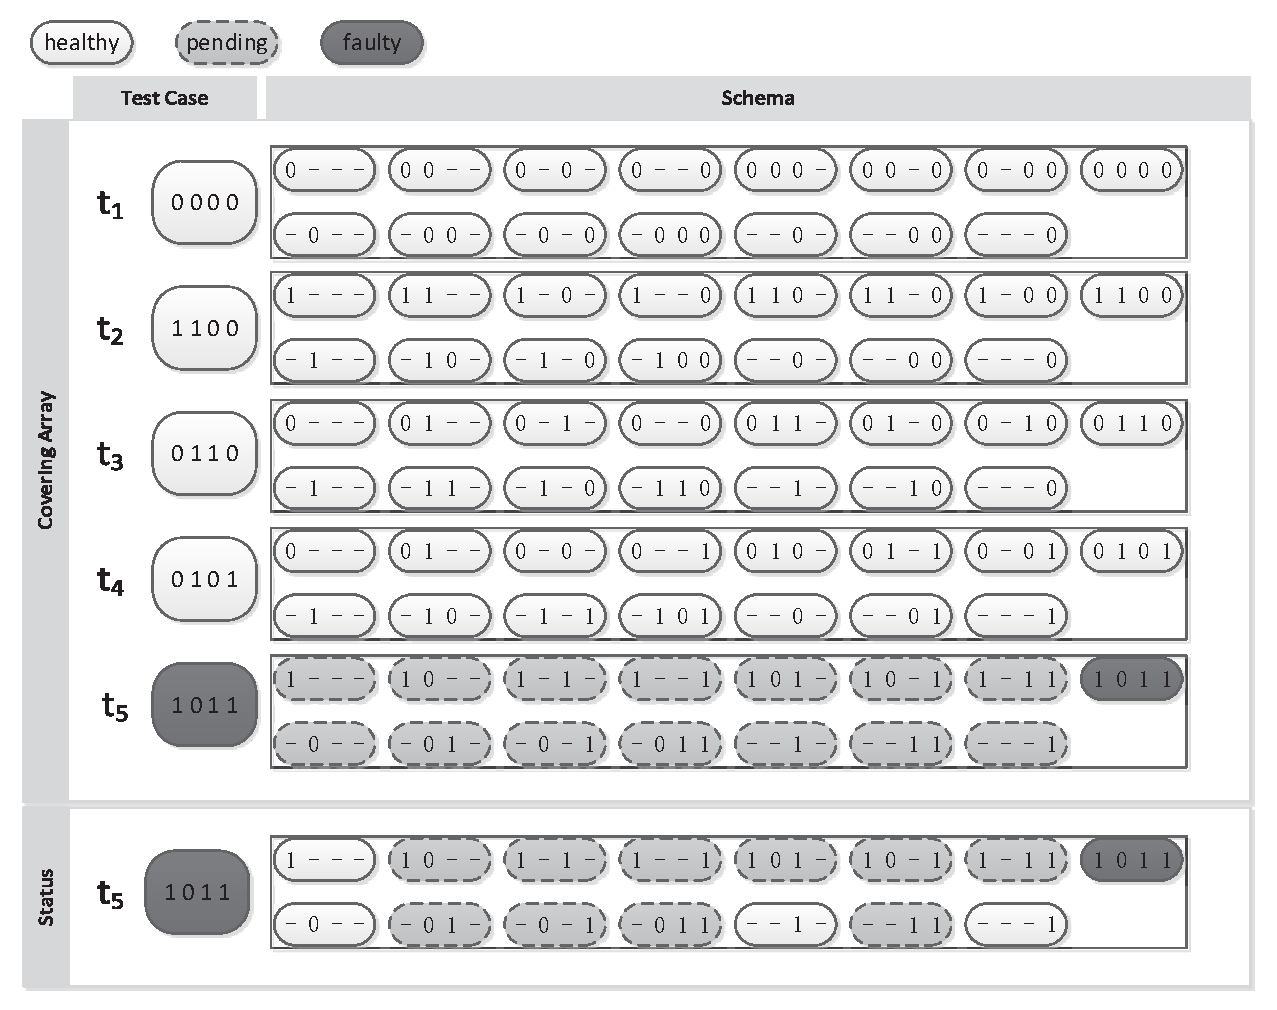
\includegraphics[width=5.6in]{ca.eps}
 \caption{The incompleteness of Covering array }
 \label{fig_inc_ca}
\end{figure*}




\subsection{The incompleteness of error locating array}
Since that , many approaches give a alleviation of how to compute the remaining schemas, which is called the fault localization. Error locating array is one of them. However, this time, we also give .

\subsection{The incompleteness of OFOT and SOFOT}
Why minimal failure-causing schema is not effective?
This example shows that . Because there still existing pending schemas.
\begin{figure*}[ht]
 \centering
 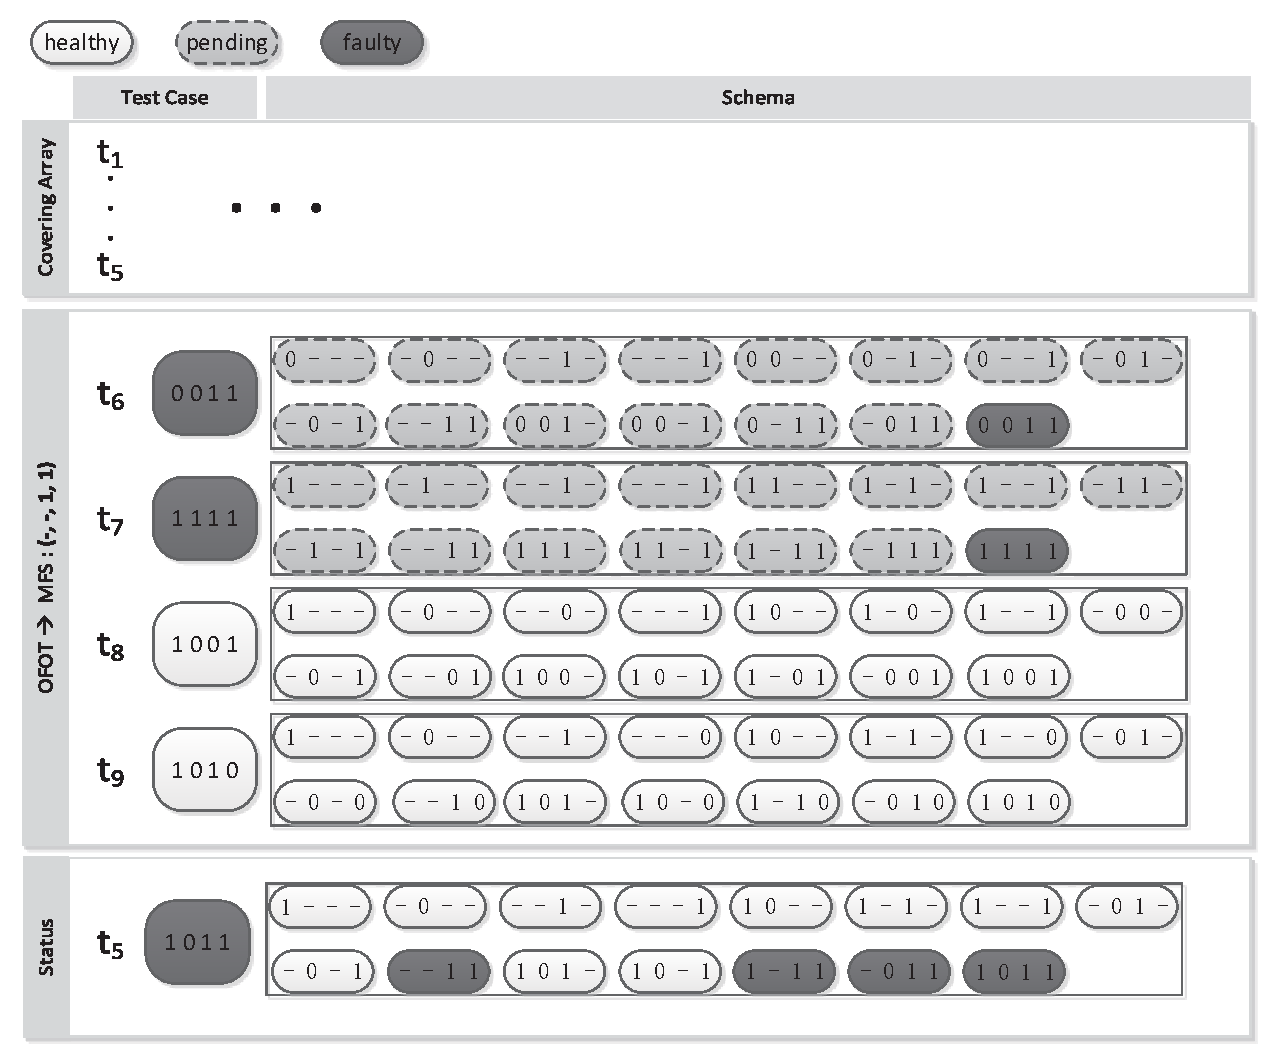
\includegraphics[width=5.6in]{ofot_single.eps}
 \caption{OFOT with single MFS}
 \label{fig_ofot_single}
\end{figure*}

\begin{figure*}[ht]
 \centering
 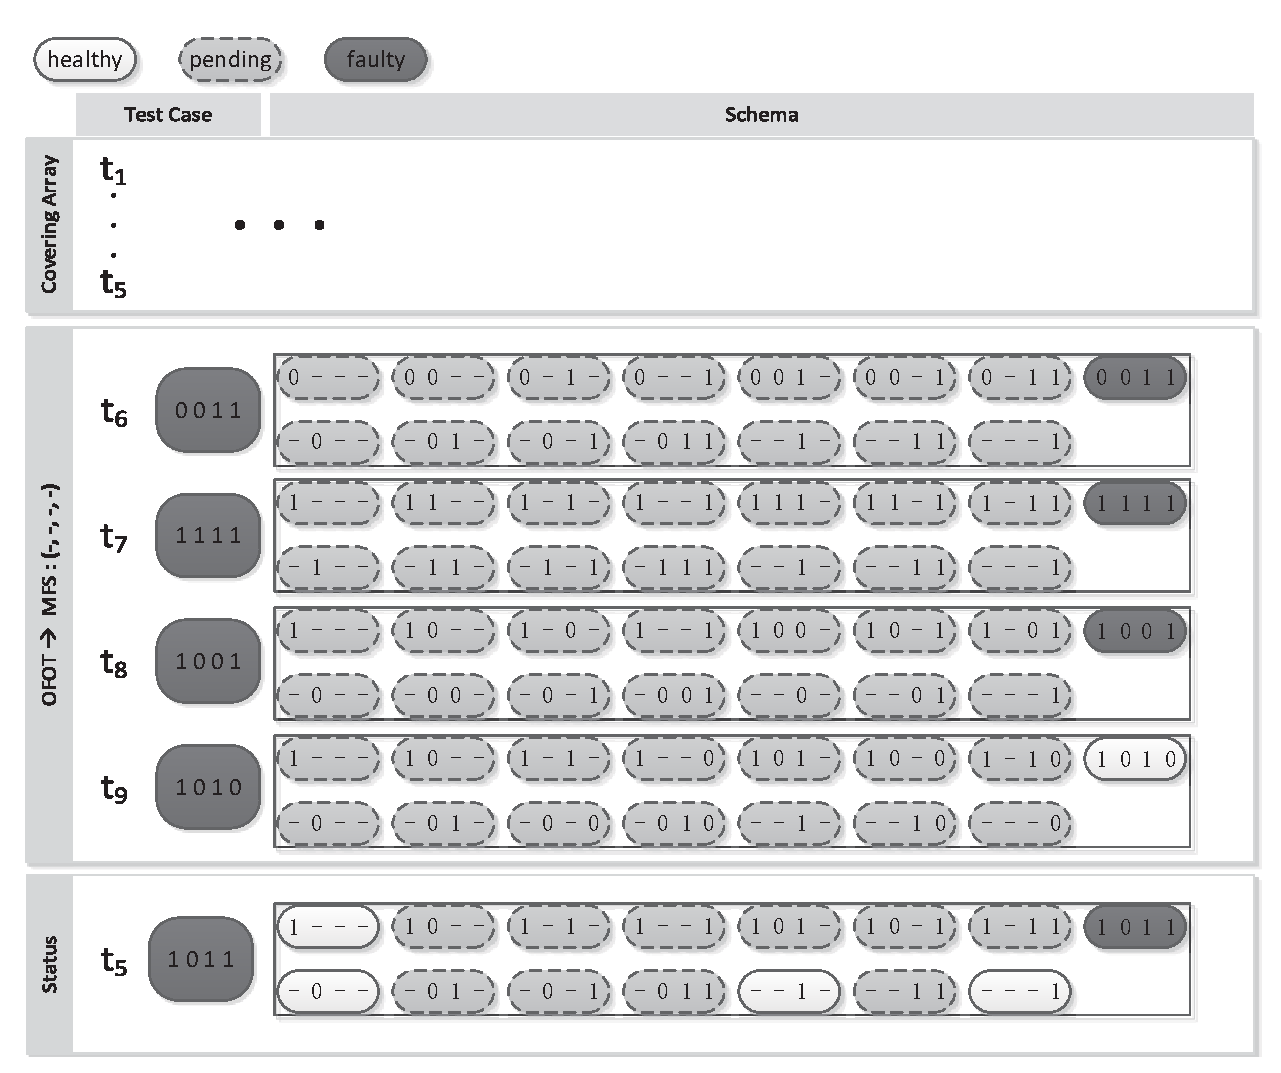
\includegraphics[width=5.6in]{ofot_multi.eps}
 \caption{OFOT with multi MFS}
 \label{fig_ofot_multi}
\end{figure*}



\subsection{The incompleteness of FIC and FIC\_BS}


Since we cannot obtain a completeness of . It is important to evaluate how incompleteness of covering array, fault localizaiton.

\begin{figure*}[!htb]
 \centering
 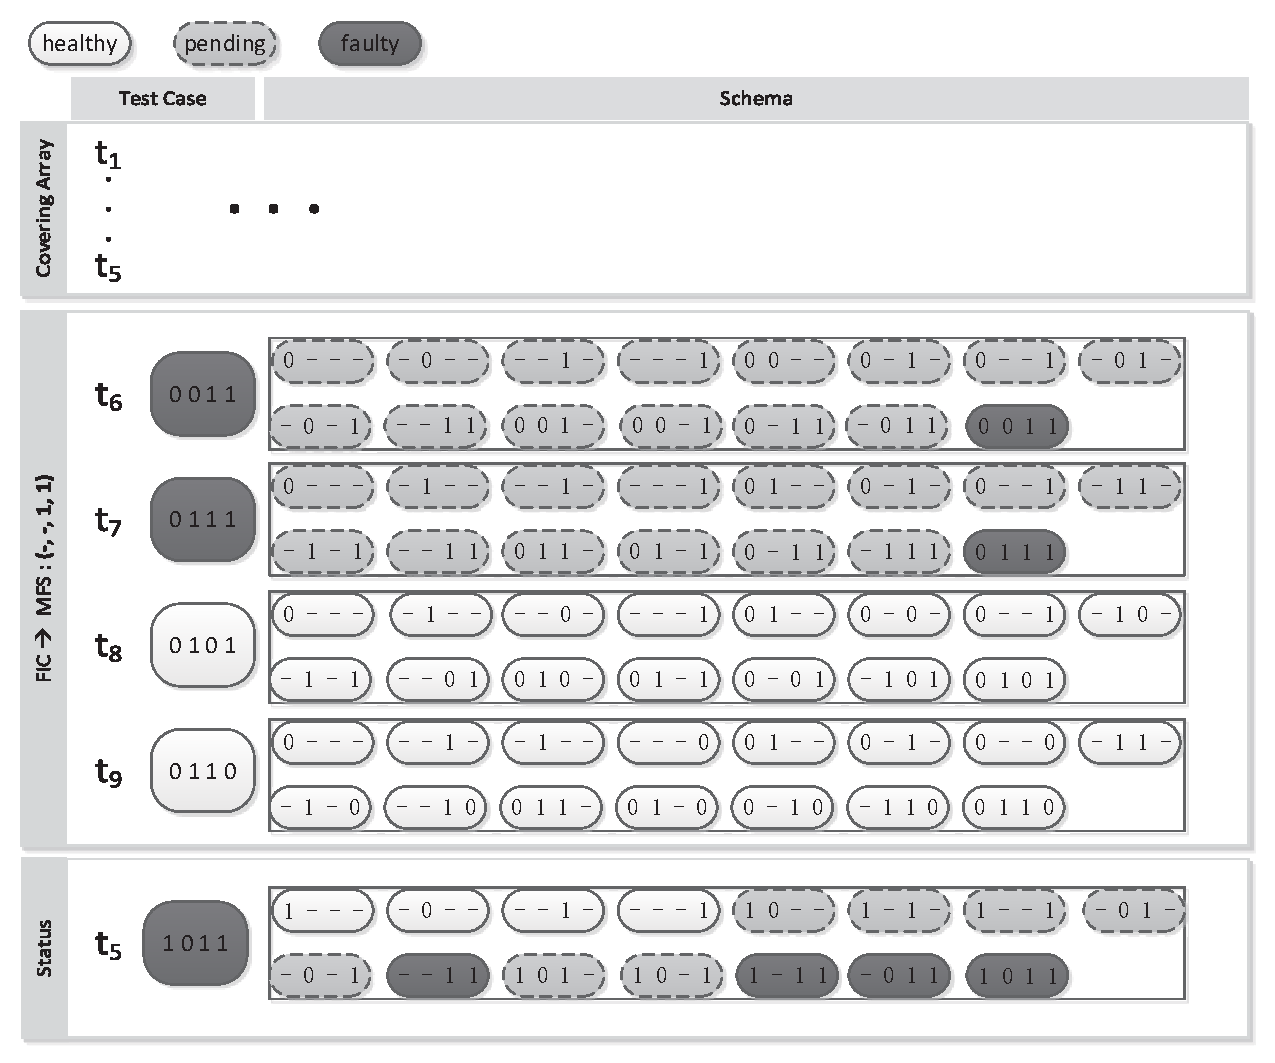
\includegraphics[width=5.3in]{fic.eps}
 \caption{fic with multiple MFS}
 \label{fig_fic_multi}
\end{figure*}


\begin{figure*}[!htb]
 \centering
 \includegraphics[width=5.3in]{finovlp.eps}
 \caption{finovlp with multiple MFS}
 \label{fig_finovlp_multi}
\end{figure*}

\subsection{A complete process}

\begin{figure*}[!htb]
 \centering
 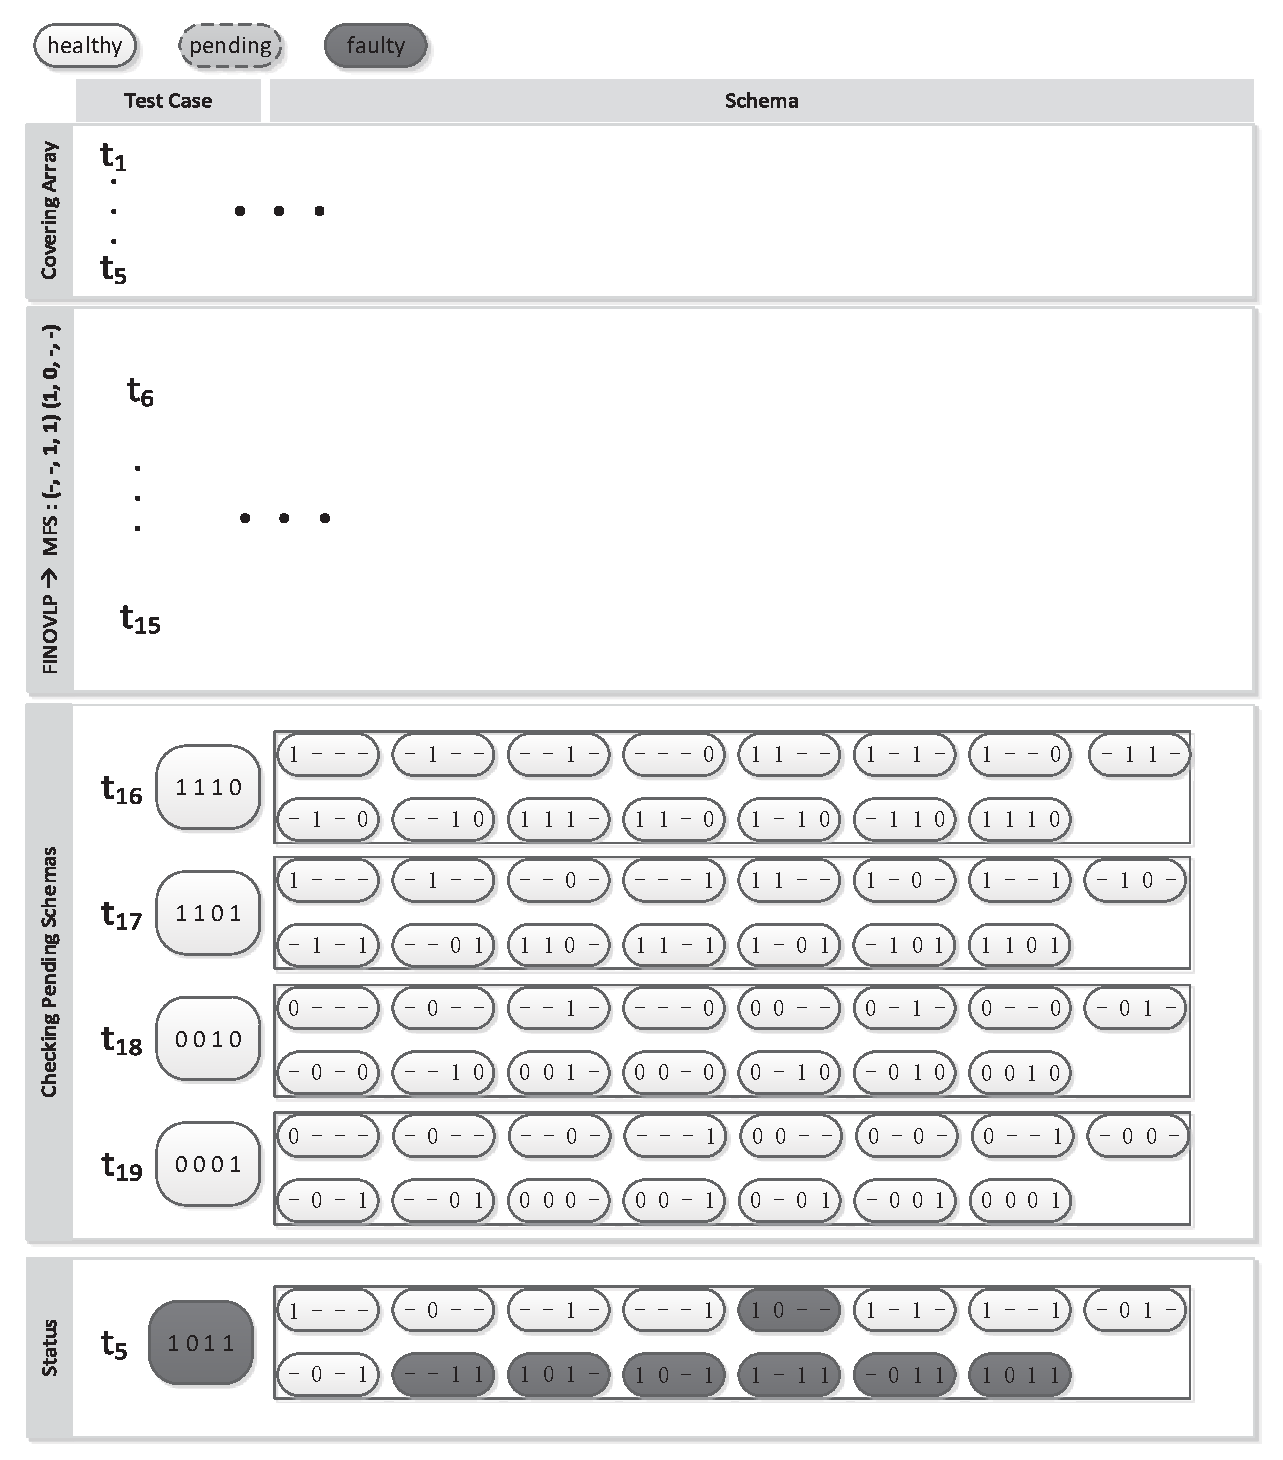
\includegraphics[width=5.3in]{non-pending.eps}
 \caption{Non pending schema}
 \label{fig_no_pending}
\end{figure*}


\section{Preliminary}\label{sec:back}
This section presents some definitions and propositions to give a formal model for CT.

%\subsection{Failure-inducing interactions in CT}

Assume that the Software Under Test (SUT) is influenced by a set of parameters $P$, which contains \emph{n} parameters, and each parameter $p_{i} \in P$ can take the values from the finite set $V_{i}$ ($i$ = 1,2,..n).

\newtheorem{assumption}{Assumption}
%\newtheorem{proposition}{Proposition}

%\newdef{definition}{Definition}
\begin{definition}\label{de:testcase}
A \emph{test case} of the SUT is a tuple of \emph{n} values, one for each parameter of the SUT. It is denoted as  ($v_{1}$, $v_{2}$,...,$v_{n}$), where $v_{1}\in V_{1}$, $v_{2} \in V_{2}$ ... $v_{n} \in V_{n}$.
\end{definition}
%a \emph{n}-tuple

In practice, these parameters in the test case can represent many factors, such as input variables, run-time options, building options or various combination of them. We need to execute the SUT with these test cases to ensure the correctness of the behaviour of the SUT.

%\begin{definition}
We consider any abnormally executing test case as a \emph{fault}. It can be a thrown exception, compilation error, assertion failure or constraint violation. When faults are triggered by some test cases, it is desired to figure out the cause of these faults.
%Some subsets of these test cases should be analysed.
%\end{definition}


\begin{definition}\label{de:schema}
For the SUT, the $\tau$-set \{$(p_{x_{1}}, v_{x_{1}})$, $(p_{x_{2}}, v_{x_{2}})$, ..., $(p_{x_{\tau}}, v_{x_{\tau}})$\}, where $0 \leq x_{i} \leq n$, $p_{x_{i}} \in P$, and $v_{x_{i}} \in V_{x_{i}}$, is called a $\tau$-degree \emph{schema} ($0 < \tau \leq n $), when a set of $\tau$ values assigned to $\tau$ distinct parameters.

For example, the interactions (Highlight: Off, Status Bar: On, Smart tags: Off) appearing in Section \ref{sec:intro} is a 3-degree schema, where three parameters are assigned to corresponding values. In effect a test case itself is a n-degree \emph{schema}, which can be described as \{$(p_{1}, v_{1})$, $(p_{2}, v_{2})$, ..., $(p_{n}, v_{n})$\}.
%Furthermore, if a test case contains a \emph{schema}, i.e., every fixed value in the schema is in this test case, we say this test case \emph{contains} the \emph{schema}.
%, which can be denoted as $k-value\  combination \in T$
\end{definition}
Note that the schema is a formal description of the interaction between parameter values we discussed before.

\begin{definition}\label{de:subsume}
Let $c_{1}$ be a \emph{l}-degree schema, $c_{2}$ be an \emph{m}-degree schema in SUT and $l < m$. If $\forall e \in c_{1}$, $e \in c_{2}$, then $c_{1}$ is the $sub-schema$ of $c_{2}$, and $c_{2}$ the $super-schema$ of $c_{2}$, which can be denoted as $c_{1} \prec c_{2}$.
\end{definition}

For example,  the 2-degree schema \{(Highlight, Off), (Status Bar, On)\} is a sub-schema of the 3-degree schema \{(Highlight, Off), (Status Bar, On), (Smart tags, Off)\}.

\begin{definition} \label{de:faulty:minimal}
If for any test cases that contain a schema, say $c$, it will trigger a failure, then we call this schema $c$ the \emph{faulty schema}. Additionally, if none of sub-schema of $c$ is a \emph{faulty schema}, we then call the schema $c$ the \emph{minimal failure-causing schema (MFS)} \cite{nie2011minimal}.

%Based on this, if a test case $t$ hit such a failure-inducing combination, say $c(F)$, it should trigger the fault $F$, for which the test case can be put as $t(F)$
\end{definition}

Note that MFS is identical to the failure-inducing interaction discussed previously. In this paper, the terms \emph{failure-inducing interactions} and \emph{MFS} are used interchangeably. Figuring the MFS helps to identify the root cause of a failure and thus facilitate the debugging process.


\begin{definition}\label{de:healthy:maximal}
A schema, say, $c$, is called a \emph{healthy schema} when we find at least one passing test case that contains this schema. In addition, if none of super-schema of $c$ is the \emph{healthy schema}, we then call the schema $c$ the \emph{maximal healthy schema (MHS)}.
\end{definition}

These two type of schemas, i.e., MFS and MHS, are the keys to our approach, as they are essentially representations of the healthy schemas and faulty schemas in a test case. As shown later, other schemas can be determined to be healthy or faulty by these two type of schemas. As a result, we just need to record these two types of schemas (normally a small amount) instead of recording all the schemas in a test case (up to $2^{n}$) when identifying MFS.

%Note that the MFS is based on the assumption that .

\begin{definition}\label{de:pending}
A schema is called a \emph{pending} schema, if it is not yet determined to be \emph{healthy} schema or \emph{faulty} schema.
\end{definition}

The \emph{pending} schema is actually the \emph{un-determined} schema discussed in Section \ref{sec:intro}. In effect, to identify the MFS in a failing test case is to figure out all the \emph{pending} schemas, and then try to classify each of them into \emph{healthy} or \emph{faulty} schema. After that, the MFS can be selected from those \emph{faulty} schemas by definition.

%\begin{definition}
%If a schema is a \emph{faulty} schema and satisfy the followed condition:
%1. None of its subschemas is \emph{faulty} schema; 2. At least one of its subschemas is \emph{pending} schema. We then call the schema a \emph{candidate minimal faulty schema} (\emph{CMXS}).
%\end{definition}
%
%\begin{definition}
%If a schema is a \emph{healthy} schema and satisfy the followed condition:
%1. None of its super-schemas are healthy schemas; 2. at least one of its subschemas is pending schema. We then call this schema a \emph{candidate maximum healthy schema} (\emph{CMNS}).
%\end{definition}

%Note that failures discussed are assumed to be deterministic in this paper.
To facilitate our discussion, we introduce the following assumptions that will be used throughout this paper:

\begin{assumption}  The execution result of a test case is deterministic.
\end{assumption}

This assumption is a common assumption of CT\cite{zhang2011characterizing,ghandehari2012identifying,niu2013identifying}. It indicates that the outcome of executing a test case is reproducible and will not be affected by some random events. Some approaches have already proposed measures to handle this problem, e.g., studies in \cite{yilmaz2006covering,fouche2009incremental} use multiple covering arrays to avoid this problem.

\begin{assumption} If a test case contains a MFS, it must fail as expected.
\end{assumption}

This assumption shows that we can always observe the failure caused by the MFS. In practice, some issues may prevent this observation. For example, the coincidental correctness problem \cite{Masri:2014:PCC:2582050.2559932} may happen through testing, when the faulty-code is executed but the failure doesn't propagate to the output. Masking effect \cite{yilmaz2013reducing} may also make the failure-observation difficult, as other failure may triggered and stop the program to go on discovering the remaining failures.

We will later discuss the impacts on MFS identification from these two assumptions, as well as how to alleviate them. Based on these definitions and assumptions, we can get several propositions as following. These propositions are the foundation of our approach, and their proofs are omitted due to their simplicity.

\begin{proposition}\label{pro:subsumetrans}
Given schemas $s_{1}$, $s_{2}$, and $s_{3}$, if $s_{1} \prec s_{2}$, $s_{2} \prec s_{3}$, then $s_{1} \prec s_{3}$.
\end{proposition}




\begin{proposition}\label{pro:superoffaulty}
Given a faulty schema $s_{1}$, then $\forall s_{2}, s_{1} \prec s_{2}$, $s_{2}$ is a faulty schema.
\end{proposition}


\begin{proposition}\label{pro:subofhealthy}
Given a healthy schema $s_{1}$, then $\forall s_{2}, s_{2} \prec s_{1}$, $s_{2}$ is a healthy schema.
\end{proposition}


\begin{proposition}\label{pro:pending}
Given two pending schemas $s_{1}$, $s_{2}$, and $s_{1} \prec s_{2}$. Then $\forall s_{3}, s_{1} \prec s_{3} \prec s_{2}$, $s_{3}$ is a pending schema.
\end{proposition}


You should give normal sentences description and examples of them (if possible, give some simple proofs)

\section{Pending schema}\label{sec:pending}
In this section, we will describe our approach to identify the failure-inducing schemas in the SUT. To give a better description, we will give several propositions which provide theoretical supports for our approach. The proofs of these propositions are given in the Appendix.

\subsection{What is pending schema}
Through the motivating examples, we can learn that the pending schema is not checked to be healthy and faulty. That is,

However, to emulate all the faulty schemas and all the healthy schemas is very large. By the propostios 3 and 4,

More formally, we can learn that it should not be any super-schemas of existing faulty schemas, and any sub-shemas of existing healthy schemas.


\subsection{Obtaining pending schema}

To identify the MFS in a failing test case, we need to figure out all the pending schemas and then classify them into faulty or healthy schemas. For this, we firstly need to be able to find one pending schema and check it. Then, we repeat this procedure until no more pending schema can be obtained.
%first describe how to obtain one pending schema.

To be general, we formalize the problem of obtaining one pending schema as the following problem:

\emph{Given a failing test case $t$ =\{$(p_{1}, v_{1})$, $(p_{2}, v_{2})$, ..., $(p_{n}, v_{n})$\}, a set of faulty schemas $FSS$ = \{ $c_{1}, c_{2}, ... c_{i}, ...$ \}, where  $c_{i} \prec t$ or $c_{i} = t$ (That is, $c_{i} \preceq t $), a set of healthy schemas $HSS$ = \{ $c_{1}, c_{2}, ... c_{i}, ...$ \}, where  $c_{i} \preceq t$, and $FSS \bigcap HSS = \emptyset$. The goal is to find one pending schema.}

Note that at the beginning of MFS identification, if there is no additional information, $FSS$ will be initialized to have one element, i.e., $t$ itself, and $HSS$ is an empty set.

We will settle this problem step by step. According to the Propositions \ref{pro:superoffaulty} and \ref{pro:subofhealthy}, it is easy to find that, the pending schemas set PSS should be the following set
\begin{equation}
\begin{aligned}\label{eq:pssfirst}
PSS=\{ c | c \prec t\ \&\&\ \forall c_{f} \in FSS,  c_{f} \npreceq c   \&\&\  \forall c_{h} \in HSS, c \npreceq c_{h} \} .
\end{aligned}
\end{equation}

To obtain one pending schema, we just need to select one schema which satisfies $ c \in PSS$. However, to directly utilize Formula \ref{eq:pssfirst} is not practical to obtain one pending schema, because in the worst case it needs to check every schema in a test case $t$, of which the complexity is O($2^{n}$). Hence, we need to find another formula which is equivalent to Formula \ref{eq:pssfirst}, but with much lower complexity.

For this purpose, we defined the following two sets, i.e. CMXS and CMNS.

\begin{definition}
For a k-degree faulty schema c = \{$(p_{x_{1}}, v_{x_{1}})$, $(p_{x_{2}}, v_{x_{2}})$, ..., $(p_{x_{k}}, v_{x_{k}})$\}, a failing test case t = \{$(p_{1}, v_{1})$, $(p_{2}, v_{2})$, ..., $(p_{n}, v_{n})$\}, and $c \preceq t$. We denote the candidate maximal pending schema set as CMXS(c,t)= \{$t \backslash (p_{x_{i}}, v_{x_{i}})$ | $(p_{x_{i}}, v_{x_{i}}) \in c $\}.
\end{definition}

Note that CMXS is the set of schemas that remove one distinct factor value in c, such that all these schemas will not be the super-schema of c. For example assume the failing test case \{$(p_{1}, v_{1})$, $(p_{2}, v_{2})$, $(p_{3}, v_{3})$, $(p_{4}, v_{4})$\}, and a faulty schema \{$(p_{1}, v_{1})$, $(p_{3}, v_{3})$\}. Then the CMXS set is \{ \{$(p_{2}, v_{2})$,  $(p_{3}, v_{3})$, $(p_{4}, v_{4})$\}, \{$(p_{1}, v_{1})$,  $(p_{2}, v_{2})$, $(p_{4}, v_{4})$\} \}. Obviously, the complexity of obtaining CMXS of one faulty schema is O($\tau$), where $\tau$ is the number of parameter values in this faulty schema, i.e., the degree of this schema.

With respect to the CMXS set of a single faulty schema, we can get the following proposition:


\begin{proposition}\label{pro:subofCMXS}
Given a faulty schema $c_{1}$, a failing test case $t$, where $c_{1} \preceq t$, we have \{$c\ |\ c \prec t\ \&\&\ c_{1} \npreceq c$\} $=$  \{$ c\ |\ \exists c_{1}' \in CMXS(c_{1}, t)$, $c \preceq c_{1}'$\}.
\end{proposition}

This proposition means that the pending schema must be the sub-schema or equal to the schemas in CMXS, otherwise, it is a faulty schema.

In the equation of Proposition \ref{pro:subofCMXS}, the schemas of the left side, i.e., \{$c\ |\ c \preceq t\ \&\&\ c_{1} \npreceq c$\}, are the sub-schemas of test case $t$, but not the super-schemas of faulty schema $c_{1}$ nor equal to $c_{1}$.  Note that the pending schemas can only appear in this set, because any schema that is not belong to this set is faulty schema according to Proposition \ref{pro:superoffaulty}. The right side set in this equation, i.e., \{$ c\ |\ \exists c_{1}' \in CMXS(c_{1}, t)$, $c \preceq c_{1}'$\}, are schemas which are sub-schemas of or equal to at least one schema in $CMXS(c_{1}, t)$. Proposition \ref{pro:subofCMXS} indicates that these two schema sets are equivalent. As an example, considering a failing test case $t$ -- \{($p_{1}$, 1),($p_{2}$, 1),($p_{3}$, 1),($p_{4}$, 1)\}, and a faulty schema $c_{f}$ --  \{($p_{3}$, 1)\}. Table \ref{examleOfCMXSPro} shows the schema set  \{$c\ |\ c \prec t\ \&\&\ c_{f} \npreceq c$\}, $CMXS(c_{f}, t)$ and \{$ c\ |\ \exists c_{1}' \in CMXS(c_{f}, t)$, $c \preceq c_{1}'$\}.

% Table generated by Excel2LaTeX from sheet 'Sheet3'
\begin{table*}[ht]
  \centering
  \setlength{\tabcolsep}{2pt}
  \caption{An example of Proposition \ref{pro:subofCMXS}}
  {\footnotesize
    \begin{tabular}{|c|c|c|c|}
    \hline
  \textbf{  Test case $\textbf{t}$} & \textbf{ \{$\textbf{c}\ |\ \textbf{c} \prec \textbf{t}\ \&\&\ \textbf{c}_{\textbf{f}} \npreceq \textbf{c}$\} }& \textbf{ CMXS($\textbf{c}_{\textbf{f}}, $\textbf{t}$ $)} & \textbf{\{$ \textbf{c}\ |\ \exists \textbf{c}_{\textbf{1}}' \in \textbf{CMXS}\textbf{(}\textbf{c}_{\textbf{f}}, \textbf{t}\textbf{)}$, $\textbf{c} \preceq \textbf{c}_{\textbf{1}}'$ \}}\\\hline
    \{($p_{1}$, 1),($p_{2}$, 1),($p_{3}$, 1),($p_{4}$, 1)\}  & \{($p_{1}$, 1),($p_{2}$, 1),($p_{4}$, 1)\} & \{($p_{1}$, 1),($p_{2}$, 1),($p_{4}$, 1)\} & \{($p_{1}$, 1),($p_{2}$, 1),($p_{4}$, 1)\}\\ \cline{1-1}
      \textbf{Faulty schema $\textbf{c}_{\textbf{f}}$}  & \{($p_{1}$, 1),($p_{2}$, 1)\} &  & \{($p_{1}$, 1),($p_{2}$, 1)\} \\\cline{1-1}
     \{($p_{3}$, 1)\}         & \{($p_{1}$, 1),($p_{4}$, 1)\}&  &\{($p_{1}$, 1),($p_{4}$, 1)\}\\
          &       \{($p_{2}$, 1),($p_{4}$, 1)\} &  &\{($p_{2}$, 1), ($p_{4}$, 1)\}\\
          &       \{($p_{1}$, 1)\} &  &\{($p_{1}$, 1)\}\\
          &       \{($p_{2}$, 1)\} &  &\{($p_{2}$, 1)\}\\
          &       \{($p_{4}$, 1)\} &  & \{($p_{4}$, 1)\}\\\hline
    \end{tabular}}%
  \label{examleOfCMXSPro}%
\end{table*}%

%
%We can find that all these schemas can be find at least one. And all the subschemas of the right side are all in the left side. For example, (12) are all the sub-schemas

%when given a faulty schema $c_{1}$ and a failing test case $t$, the pending schemas can only appeared in set \{$c\ |\ \exists c_{1}' \in CMXS(c_{1}, t), c \preceq c_{1}'$\}.

We can extend this conclusion to a set of faulty schemas. For this, we need the following notation: For two faulty schemas $c_{1}$, $c_{2}$, and a failing test case $t$ ($c_{1} \preceq t$, $c_{2} \preceq t$), let $CMXS(c_{1}, t) \bigwedge CMXS(c_{2}, t)  = \{ c\ |\ c = c_{1}' \cap c_{2}',\ where\ c_{1}' \in CMXS(c_{1}, t),\ and\ c_{2}' \in CMXS(c_{2}, t) \}$.

For example, let $t$ = \{$(p_{1},v_{1}), (p_{2}, v_{2}), (p_{3}, v_{3})$\}, $c_{1}$ = \{$(p_{1}$ $, v_{1}), (p_{2}, v_{2})$\}, $c_{2}$ = \{$(p_{2}, v_{2}), (p_{3}, v_{3})$\}. Then we have $CMXS$ $(c_{1}, t)$ = \{ \{$(p_{1}, v_{1}), (p_{3}, v_{3})$\}, \{$(p_{2}, v_{2}), (p_{3}, v_{3})$\} \}, $CMXS(c_{2},$ $ t)$ = \{ \{$(p_{1}, v_{1}), (p_{2}, v_{2})$\}, \{$(p_{1}, v_{1}), (p_{3}, v_{3})$\} \}, and  $CMXS(c_{1},$ $ t) \bigwedge CMXS(c_{2}, t) = \{ \{(p_{1}, v_{1})\},$ $ \{(p_{1}, v_{1}), $ $(p_{3}, v_{3})\}, $ $ \{(p_{2}, v_{2})\}, $ $\{(p_{3}, v_{3})\} \} $. It is easy to know the complexity of obtaining CMXS of two faulty schemas is O($\tau^{2}$), where $\tau$ is the number of parameter values in the faulty schema. Based on this, we denote $CMXS(FSS,t)$ for a set of faulty schemas.

\begin{definition}
Given a failing test case t = \{$(p_{1}, v_{1})$, $(p_{2}, v_{2})$, ..., $(p_{n}, v_{n})$\}, and a set of faulty schemas FSS = \{$c_{1} , c_{2}, ... c_{i}, ...$\}, where $ c_{i} \preceq t$,  we denote the candidate maximal pending schema of this set as CMXS(FSS,t)= $\bigwedge_{c_{i}\in FSS} CMXS(c_{i}, t)$.
\end{definition}

Note to compute the CMXS of a set of faulty schema, we just need to sequentially compute the CMXS of two faulty schemas until the last schema in this set is computed. Hence, the complexity of obtaining CMXS of a set of faulty schema is O($\tau^{|FSS|}$), where |FSS| is the number of faulty schemas in the schema set, and $\tau$ is the degree of the schema. According to Proposition \ref{pro:subofCMXS}, we have:

\begin{proposition}\label{pro:subofCMXSfor2}
Given a failing test case t = \{$(p_{1}, v_{1})$, $(p_{2}, v_{2})$, ..., $(p_{n}, v_{n})$\}, and a set of faulty schemas FSS = \{$c_{1} , c_{2}, ... c_{i}, ...$\}, where $ c_{i} \preceq t$,  we have \{$c\ |\ c \preceq t\ \&\&\ \forall c_{i} \in FSS, c_{i} \npreceq c $\} $=$  \{$ c\ |\ \exists c_{1}' \in CMXS(FSS, t)$, $c \preceq c_{1}'$\}.
\end{proposition}

Proposition \ref{pro:subofCMXSfor2} extends Proposition \ref{pro:subofCMXS} from a single faulty schema to a set of faulty schemas.

As an example, considering a failing test case $t$ -- \{($p_{1}$, 1),($p_{2}$, 1),($p_{3}$, 1),($p_{4}$, 1)\}, and a set of faulty schemas  $FSS$ -- \{ \{($p_{3}$, 1)\},  \{($p_{1}$, 1), ($p_{2}$, 1)\} \}. Table \ref{examleOfCMXSPro2} shows the schema set \{$c\ |\ c \prec t\ \&\&\ \forall c_{i} \in FSS, c_{i} \npreceq c $\}, $CMXS(FSS, t)$ and \{$ c\ |\ \exists c_{1}' \in CMXS(FSS, t)$, $c \preceq c_{1}'$\}.

% Table generated by Excel2LaTeX from sheet 'Sheet3'

\begin{table*}[ht]
  \centering
  \setlength{\tabcolsep}{2pt}
  \caption{An example of Proposition \ref{pro:subofCMXSfor2}}
  {\footnotesize
    \begin{tabular}{|c|c|c|c|}
    \hline
  \textbf{  Test case $\textbf{t}$} & \textbf{ \{$\textbf{c}\ |\ \textbf{c} \prec \textbf{t}\ \&\&\ \forall \textbf{c}_{\textbf{i}} \in FSS, \textbf{c}_{\textbf{i}} \npreceq \textbf{c}$\} }& \textbf{  CMXS(FSS, t)} & \textbf{\{$ \textbf{c}\ |\ \exists \textbf{c}_{\textbf{1}}' \in \textbf{ CMXS(FSS, t)} $ , $\textbf{c} \preceq \textbf{c}_{\textbf{1}}'$ \}}\\\hline
    \{($p_{1}$, 1),($p_{2}$, 1),($p_{3}$, 1),($p_{4}$, 1)\}  & \{($p_{1}$, 1),($p_{4}$, 1)\} & \{($p_{1}$, 1),($p_{4}$, 1)\} & \{($p_{1}$, 1),($p_{4}$, 1)\}\\ \cline{1-1}
      \textbf{Faulty schema set FSS}  & \{($p_{2}$, 1),($p_{4}$, 1)\} &  \{($p_{2}$, 1),($p_{4}$, 1)\} & \{($p_{2}$, 1),($p_{4}$, 1)\} \\\cline{1-1}
     \{($p_{3}$, 1)\}         & \{($p_{1}$, 1)\}&  &\{($p_{1}$, 1)\}\\
     \{($p_{1}$, 1),($p_{2}$, 1)\}  &       \{($p_{2}$, 1)\} &  &\{($p_{2}$, 1)\}\\
          &       \{($p_{4}$, 1)\} &  & \{($p_{4}$, 1)\}\\\hline
    \end{tabular}}%
  \label{examleOfCMXSPro2}%
\end{table*}%
%
%\begin{proof}
%
%\end{proof}
%Based on previous propositions, we can get that the pending schemas can only appeared in set $P_{up}$ = \{$c\ |\ \exists c_{1}' \in CMXS(FSS,t), c \preceq c_{1}'$\}.


Next, we give the definition of \emph{CMNS}.

\begin{definition}
For a k-degree healthy schema c = \{$(p_{x_{1}}, v_{x_{1}})$, $(p_{x_{2}}, v_{x_{2}})$, ..., $(p_{x_{k}}, v_{x_{k}})$\}, a failing test case t = \{$(p_{1}, v_{1})$, $(p_{2}, v_{2})$, ..., $(p_{n}, v_{n})$\}, and $c \prec t$. We denote the candidate minimal pending schema set as CMNS(c,t)=\{$\{(p_{x_{i}}, v_{x_{i}})\}$ | $(p_{x_{i}}, v_{x_{i}}) \in t \backslash c $\}.
\end{definition}

Note that CMNS is the set of schemas that are assigned to one distinct factor value that is not in c, such that all these schemas will not be the sub-schema of c. For example assume the failing test case \{$(p_{1}, v_{1})$, $(p_{2}, v_{2})$, $(p_{3}, v_{3})$, $(p_{4}, v_{4})$\}, and a healthy schema \{$(p_{1}, v_{1})$, $(p_{3}, v_{3})$\}. Then the CMNS set is \{ \{$(p_{2}, v_{2})$\}, \{$(p_{4}, v_{4})$\} \}.  With respect to the CMNS set of a single healthy schema, we can get the following proposition:

\begin{proposition}\label{pro:superofCMNS}
Given a healthy schema $c_{1}$, a failing test case $t$, where $c_{1} \prec t$, we have \{$c\ |\ c \prec t\ \&\&\ c \npreceq c_{1}$\} $=$  \{$ c\ |\ c \prec t \  \&\& \ \exists c_{1}' \in CMNS(c_{1}, t)$, $c_{1}' \preceq c$\}.
\end{proposition}

This proposition means that the pending schema must be the super-schema or equal to the schemas in CMNS, otherwise, it is a healthy schema.

In the equation of Proposition \ref{pro:superofCMNS}, the schemas of the left side, i.e., \{$c\ |\ c \preceq t\ \&\&\ c \npreceq c_{1}$\}, are the sub-schemas of test case $t$, but not the sub-schemas of healthy schema $c_{1}$ nor equal to $c_{1}$.  It is obvious that the pending schemas can also only appear in this set, because they cannot be the sub-schema of any healthy schema nor equal to them. The right side set in this equation, i.e.,\{$ c\ |\ c \preceq t \  \&\& \ \exists c_{1}' \in CMNS(c_{1}, t)$, $c_{1}' \preceq c$\}, are sub-schemas of test case $t$, and also are the super-schemas of or equal to at least one schema in $CMXS(c_{1}, t)$. Proposition \ref{pro:superofCMNS} indicates that these two schema sets are equivalent. As an example, considering a failing test case $t$ -- \{($p_{1}$, 1),($p_{2}$, 1),($p_{3}$, 1),($p_{4}$, 1)\}, and a healthy schema $c_{h}$ --  \{($p_{1}$, 1),($p_{2}$, 1),($p_{3}$, 1)\}. Table \ref{examleOfCMNSPro} shows the schema set  \{$c\ |\ c \prec t\ \&\&\ c_{h} \npreceq c$\}, $CMNS(c_{h}, t)$ and {$ c\ |\ c \prec t\ \&\& \ \exists c_{1}' \in CMXS(c_{h}, t)$, $c_{1}' \preceq c$\}.

% Table generated by Excel2LaTeX from sheet 'Sheet3'
\begin{table*}[ht]
  \centering
  \setlength{\tabcolsep}{2pt}
  \caption{An example of Proposition \ref{pro:superofCMNS}}
  {\footnotesize
    \begin{tabular}{|c|c|c|c|}
    \hline
  \textbf{  Test case $\textbf{t}$} & \textbf{ \{$\textbf{c}\ |\ \textbf{c} \prec \textbf{t}\ \&\&\ \textbf{c} \npreceq \textbf{c}_{\textbf{h}}$\} }& \textbf{ CMNS($\textbf{c}_{\textbf{h}}$, $\textbf{t}$)} & \textbf{\{$ \textbf{c}\ |\ \textbf{c} \prec \textbf{t} \ \&\& \ \exists \textbf{c}_{\textbf{1}}' \in \textbf{CMNS}\textbf{(}\textbf{c}_{\textbf{h}}, \textbf{t}\textbf{)}$, $  \textbf{c}_{\textbf{1}}' \preceq \textbf{c}$ \}}\\\hline
    \{($p_{1}$, 1),($p_{2}$, 1),($p_{3}$, 1),($p_{4}$, 1)\}  & \{($p_{4}$, 1)\} & \{($p_{4}$, 1)\} & \{(($p_{4}$, 1)\}\\ \cline{1-1}
      \textbf{Heathy schema $\textbf{c}_{\textbf{h}}$}  & \{($p_{1}$, 1),($p_{4}$, 1)\} &  & \{($p_{1}$, 1),($p_{4}$, 1)\} \\\cline{1-1}
     \{($p_{1}$, 1),($p_{2}$, 1),($p_{3}$, 1)\}         &\{($p_{2}$, 1),($p_{4}$, 1)\}  &  & \{($p_{2}$, 1),($p_{4}$, 1)\}  \\
                         &\{$p_{3}$, 1),($p_{4}$, 1)\}   &  & \{$p_{3}$, 1),($p_{4}$, 1)\}  \\
                         &\{($p_{1}$, 1),($p_{2}$, 1),($p_{4}$, 1)\}   &  & \{($p_{1}$, 1),($p_{2}$, 1),($p_{4}$, 1)\}  \\
                         &\{($p_{1}$, 1),($p_{3}$, 1),($p_{4}$, 1)\}  &  & \{($p_{1}$, 1),($p_{3}$, 1),($p_{4}$, 1)\}  \\
                         &\{($p_{2}$, 1),($p_{3}$, 1),($p_{4}$, 1)\}  &  & \{($p_{2}$, 1),($p_{3}$, 1),($p_{4}$, 1)\}  \\ \hline
    \end{tabular}}%
  \label{examleOfCMNSPro}%
\end{table*}%


Similarly, for two healthy schemas $c_{1}$, $c_{2}$, and a failing test case $t$ ($c_{1} \preceq t$, $c_{2} \preceq t$), let $CMNS(c_{1}, t) \bigvee $ $CMNS(c_{2}, t)  = \{ c\ |\ c = c_{1}' \cup c_{2}',\ where\ c_{1}' \in CMXS(c_{1}, t),\ and\ c_{2}' \in CMXS(c_{2}, t) \}$.

For example, let $t$ = \{$(p_{1},v_{1}), (p_{2}, v_{2}), (p_{3}, v_{3})$\}, $c_{1}$ = \{$(p_{1}$ $, v_{1}), (p_{2}, v_{2})$\}, $c_{2}$ = \{$(p_{2}, v_{2}), (p_{3}, v_{3})$\}. Then we have $CMNS$ $(c_{1}, t)$ = \{ \{$(p_{3}, v_{3})$\} \}, $CMNS(c_{2},$ $ t)$ = \{ \{$(p_{1}, v_{1})$\} \}, and  $CMNS(c_{1},$ $ t) \bigvee CMNS(c_{2}, t) = \{ \{(p_{1}, v_{1}), (p_{3}, v_{3})\} \} $. Based on this, we denote $CMNS(HSS,t)$ for a set of faulty schemas.


\begin{definition}
Given a failing test case t = \{$(p_{1}, v_{1})$, $(p_{2}, $ $v_{2})$, ..., $(p_{n}, v_{n})$\}, and a set of healthy schemas HSS = \{$c_{1} , c_{2},$ $  ...c_{i}, ...$\}, where $ c_{i} \preceq t$, we denote the candidate minimal pending schema of this set as CMNS(HSS,t)= $ $ $\bigvee_{c_{i}\in HSS}$ $ CMNS(c_{i}, t)$.
\end{definition}

Similar to CMXS(FSS,t), the complexity to obtain CMNS(HSS,t) is O($\tau^{|HSS|}$), where |HSS| is the number of healthy schemas in the schema set, and $\tau$ is the degree of the schema. With respect to CMNS(HSS,t), we have:

\begin{proposition}\label{pro:superofCMNS2}
Given a failing test case t = \{$(p_{1}, v_{1})$, $(p_{2}, v_{2})$, ..., $(p_{n}, v_{n})$\}, and a set of healthy schemas HSS = \{$c_{1} , c_{2}, ... c_{i}, ...$\}, where $ c_{i} \preceq t$,  we have \{$c\ |\ c \prec t\ \&\&\ \forall c_{i} \in HSS, c \npreceq c_{i} $\} $=$  \{$ c\ |\ c \prec t \ \&\& \ \exists c_{1}' \in CMNS(HSS, t)$, $c_{1}' \preceq c$\}.
\end{proposition}

Similar to Proposition \ref{pro:subofCMXS} and \ref{pro:subofCMXSfor2},  Proposition \ref{pro:superofCMNS2} extends Proposition \ref{pro:superofCMNS} from a single healthy schema to a set of healthy schemas.

As an example, considering a failing test case $t$ -- \{($p_{1}$, 1),($p_{2}$, 1),($p_{3}$, 1),($p_{4}$, 1)\}, and a set of schema schemas  $HSS$ -- \{ \{($p_{1}$, 1),($p_{2}$, 1),($p_{3}$, 1)\},  \{($p_{3}$, 1),($p_{4}$, 1)\} \}. Table \ref{examleOfCMNSPro2} shows the schema set \{$c\ |\ c \prec t\ \&\&\ \forall c_{i} \in HSS, c \npreceq c_{i} $\}, $CMNS(HSS, t)$ and \{$ c\ |\ c \prec t \ \&\& \ \exists c_{1}' \in CMNS(HSS, t)$, $c_{1}' \preceq c$\}.

% Table generated by Excel2LaTeX from sheet 'Sheet3'

\begin{table*}[ht]
  \centering
  \setlength{\tabcolsep}{1pt}
  \caption{An example of Proposition \ref{pro:superofCMNS2}}
  {\footnotesize
    \begin{tabular}{|c|c|c|c|}
    \hline
  \textbf{  Test case $\textbf{t}$} & \textbf{ \{$\textbf{c}\ |\ \textbf{c} \prec \textbf{t}\ \&\&\ \forall \textbf{c}_{\textbf{i}} \in \textbf{HSS}, \textbf{c} \npreceq \textbf{c}_{\textbf{i}} $\} }& \textbf{  CMNS(HSS, t)} & \textbf{\{$ \textbf{c}\ |\ \textbf{c} \prec \textbf{t} \ \&\& \ \exists \textbf{c}_{\textbf{1}}' \in \textbf{CMNS(HSS, t)}$, $\textbf{c}_{\textbf{1}}' \preceq \textbf{c}$\}}\\\hline
    \{($p_{1}$, 1),($p_{2}$, 1),($p_{3}$, 1),($p_{4}$, 1)\}  & \{($p_{1}$, 1),($p_{4}$, 1)\} & \{($p_{1}$, 1),($p_{4}$, 1)\} & \{($p_{1}$, 1),($p_{4}$, 1)\}\\ \cline{1-1}
      \textbf{Heathy schema set HSS}  & \{($p_{2}$, 1),($p_{4}$, 1)\} & \{($p_{2}$, 1),($p_{4}$, 1)\} & \{($p_{2}$, 1),($p_{4}$, 1)\} \\\cline{1-1}
     \{($p_{1}$, 1),($p_{2}$, 1),($p_{3}$, 1)\}         &\{($p_{1}$, 1),($p_{2}$, 1),($p_{4}$, 1)\}  &  &  \{($p_{1}$, 1),$p_{2}$, 1),($p_{4}$, 1)\}   \\
     \{($p_{3}$, 1),($p_{4}$, 1)\}         &\{($p_{1}$, 1),($p_{3}$, 1),($p_{4}$, 1)\}    &  &  \{($p_{1}$, 1),($p_{3}$, 1),($p_{4}$, 1)\}  \\
                         &\{($p_{2}$, 1),($p_{3}$, 1),($p_{4}$, 1)\}   &  & \{($p_{2}$, 1),($p_{3}$, 1),($p_{4}$, 1)\}   \\ \hline
    \end{tabular}}%
  \label{examleOfCMNSPro2}%
\end{table*}%


Based on Proposition \ref{pro:subofCMXSfor2} and \ref{pro:superofCMNS2}, we can easily learn that \{$c\ |\ c \prec t\ \&\&\ \forall c_{i} \in FSS, c_{i} \npreceq c $\} $\bigcap$ \{$c\ |\ c \prec t\ \&\&\ \forall c_{i} \in HSS, c \npreceq c_{i} $\}  $=$  \{$ c\ |\ \exists c_{1}' \in CMXS(FSS, t)$, $c \preceq c_{1}'$\} $\bigcap$  \{$ c\ |\ c \prec t \ \&\& \ \exists c_{1}' \in CMNS(HSS, t)$, $c_{1}' \preceq c$\}. Considering $\forall c \in $\{$ c\ |\ \exists c_{1}' \in CMXS(FSS, t)$, $c \preceq c_{1}'$\}, $c \prec t$, we can transform the aforementioned formula into the following equation.

\{$c\ |\ c \prec t\ \&\&\ \forall c_{i} \in FSS, c _{i} \npreceq c \&\&\ \forall c_{i} \in HSS, c \npreceq c_{i}  $\} $=$  \{$ c\ |\ \exists c_{1}' \in CMXS(FSS, t)$, $c \preceq c_{1}'$ $\&\&$ $\exists c_{1}' \in CMNS(HSS, t)$, $c_{1}' \preceq c$\} $=$  \{$ c\ |\ \exists c_{1}' \in CMXS(FSS, t), c_{2}' \in CMXS(FSS, t)$, $c_{2}' \preceq c \preceq c_{1}'$ \}.

Note that the leftmost side of this equation is identical to Formula \ref{eq:pssfirst}, hence, we can learn that

%\begin{equation}\label{eq:psssecond}
%\begin{aligned}
%PSS = & \{ c\ |\ \exists c_{1}' \in CMXS(FSS, t), c \preceq c_{1}' \\
%    & \&\& \exists c_{1}' \in CMNS(HSS, t), c_{1}' \preceq c\}.
%\end{aligned}
%%PSS = \{ c\ |\ \exists c_{1}' \in CMNS(HSS, t), c_{1}' \preceq c \&\& \exists c_{1}' \in CMNS(HSS, t), c_{1}' \preceq c\}.
%\end{equation}

%Further

\begin{equation}\label{eq:psssecond}
\begin{aligned}
PSS =  \{ c\ |\ \exists c_{1}' \in CMXS(FSS, t), c_{2}' \in CMNS(HSS, t),  c_{2}' \preceq c \preceq c_{1}' \}.
\end{aligned}
%PSS = \{ c\ |\ \exists c_{1}' \in CMNS(HSS, t), c_{1}' \preceq c \&\& \exists c_{1}' \in CMNS(HSS, t), c_{1}' \preceq c\}.
\end{equation}

According to Formula \ref{eq:psssecond}, the complexity of obtaining one pending schema is O($ \tau^{|FSS|} \times \tau^{|HSS|}$). This is because to obtain one pending schema, we only need to search the schemas in $CMXS(FSS, t)$ and $CMNS(HSS, t)$, of which the complexity are O($\tau^{|FSS|}$) and O($\tau^{|HSS|}$), respectively. Then we need to check each pair of schemas in these two sets, to find whether exists $c_{1} \in CMXS(FSS, t)$, $c_{2} \in CMNS(HSS, t)$, such that $c_{2} \preceq c_{1}$. If so, then both $c_{2}$ and $c_{1}$ satisfy Formula \ref{eq:psssecond}. Furthermore, $\forall c_{3}, c_{2} \preceq c_{3} \preceq c_{1}$, $c_{3}$ also satisfy Formula \ref{eq:psssecond}. Hence, the complexity of obtaining one pending schema is O($\tau^{|FSS|} \times \tau^{|HSS|}$).

In fact, we can further reduce the complexity of obtaining pending schemas. When given a set of schemas $S$, let the minimal schemas as $S^{\bot } = \{ c | c \in S, \nexists c' \in S, c' \prec c \}$ and the maximal schemas as $S^{\top } = \{ c | c \in S, \nexists c' \in S, c \prec c' \}$. Based on this, we can have the following proposition:

\begin{proposition}\label{pro:identicialPending}
Given a failing test case $t$, a set of faulty schemas $FSS$, and a set of healthy schemas $HSS$, we have \{$ c\ |\ \exists c_{1}' \in CMXS(FSS^{\bot}, t)$, $ c_{2}' \in CMNS($ $HSS^{\top}, t)$, $c_{2}' \preceq c \preceq c_{1}'$ \} $=$  \{$ c\ |\ \exists c_{1}' \in CMXS(FSS, t)$, $c_{1}' \in CMNS(HSS, t)$, $c_{2}' \preceq c \preceq c_{1}'$ \}.
\end{proposition}

As an example, consider a failing test case $t = \{(p_{1}, 1),$ $ (p_{2}, 1), (p_{3}, 1), (p_{4}, 1)\}$, the faulty schema set $FSS =$ \{ $\{(p_{1}, $ $1), (p_{2}, 1), (p_{3}, 1)\}$, $\{(p_{1}, 1), (p_{2}, 1)\}$ \}, and the healthy schema set $HSS =$  \{ $\{(p_{2}, 1),$ $(p_{3}, 1),$ $(p_{4}, 1)\}$, $\{(p_{2}, 1), (p_{3}, 1)\}$ \}. It is easy to learn that the minimal faulty schema set $FSS^{\bot} = \{\{(p_{1}, 1), (p_{2}, 1)\}\}$, and the maximal healthy schema set $HSS^{\top}$ $= \{\{ (p_{2}, 1), (p_{3}, 1), (p_{4}, 1) \}\}$.

Fig \ref{fig_minmax} lists all the faulty schemas, healthy schemas, and pending schemas of test case $t$. At the second part, it lists the $CMXS(FSS, t)$, $CMNS(HSS, t)$, and the schema set \{$ c\ |\ \exists c_{1}' \in CMXS(FSS, t)$, $c_{1}' \in CMNS(HSS, t)$, $c_{2}' \preceq c \preceq c_{1}'$ \}. At last it shows $CMXS(FSS^{\bot}, t)$, $CMNS(HSS^{\top}, t)$ and  \{$ c\ |\ \exists c_{1}' \in CMXS(FSS^{\bot}, t)$, $ c_{2}' \in CMNS($ $HSS^{\top}, t)$, $c_{2}' \preceq c \preceq c_{1}'$ \}.

We can learn that these two schema set mentioned in Proposition \ref{pro:identicialPending} are identical in Fig \ref{fig_minmax}, but the schema set based on $CMXS(FSS^{\bot}, t)$, $CMNS(HSS^{\top}, t)$ used much fewer schemas (3 in total) to obtain the result than the schema set based on $CMXS(FSS, t)$, $CMNS(HSS, t)$ (7 in total). Another observation from this figure is that these two schema set are both identical to the pending schemas. It suggests that using CMXS and CMNS can effectively and efficiently to get the pending schemas, when compared to list all the schemas in a test case and find the pending schema one by one according to Formula \ref{eq:pssfirst}.

\begin{figure*}[ht]
 \centering
 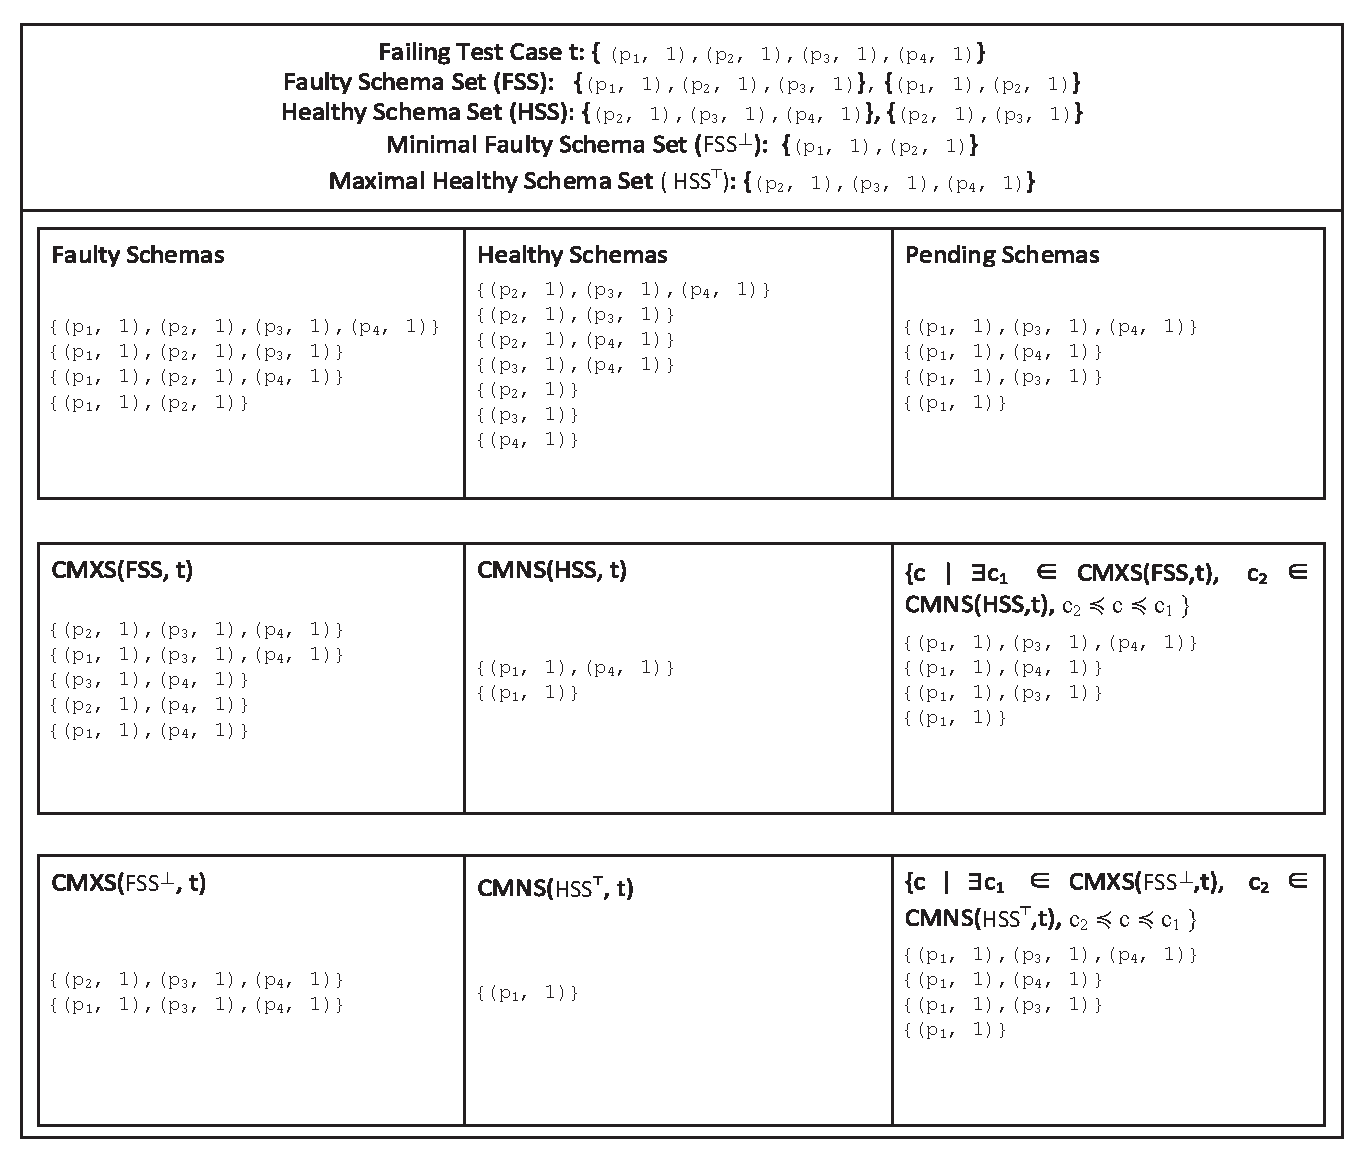
\includegraphics[width=5.6in]{minmax.eps}
 \caption{The example of Proposition \ref{pro:identicialPending}}
 \label{fig_minmax}
\end{figure*}


At last, according to Proposition \ref{pro:identicialPending}, we have the third formula to compute pending schemas as follow:

\begin{equation}\label{eq:pssthird}
\begin{aligned}
PSS =  \{ c\ |\ \exists c_{1}' \in CMXS(FSS^{\bot}, t), c_{2}' \in CMNS(HSS^{\top}, t), c_{2}' \preceq c \preceq c_{1}' \}.
\end{aligned}
%PSS = \{ c\ |\ \exists c_{1}' \in CMNS(HSS, t), c_{1}' \preceq c \&\& \exists c_{1}' \in CMNS(HSS, t), c_{1}' \preceq c\}.
\end{equation}

According to Formula \ref{eq:pssthird}, the complexity of obtaining one pending schema is O($ \tau^{|FSS^{\bot}|} \times \tau^{|HSS^{\top}|}$), where $|FSS^{\bot}|$ and $|HSS^{\top}|$ are two relatively small numbers during MFS identification.

\subsection{Getting back to the motivation example}
When applying this analysis, we can get back to the motivation example.
We do not need list all the schemas, but we can figure out which one is the pending schema (Covering array, OFOT, OFOT with single  MFS, FIC, FIC with multiple )


% Start of "Sample References" section

\section{Empirical studies}\label{sec:emp}


\subsection{The pending schemas for covering arrays}

subjects (30 existing wildly used)

generation approaches (ipog, aetg, augmented simulating?)

\subsection{The existence of pending schemas for different MFS identification approaches}

subjects (my , may also used from )

approaches (my)

\subsection{The characteristics of pending schemas with various types of MFS (multiple, overlapped, single, low-high degrees)}

the same as the captions


\subsection{The effectiveness of the approach}

three way: (three formulas in the propositions)


\subsection{Threats to validity}


\section{Discussion}\label{sec:discussion}


\section{Related works}\label{sec:related}
Shi and Nie \cite{shi2005software} presented an approach for failure revealing and failure diagnosis in CT , which first tests the SUT with a covering array, then reduces the value schemas contained in the failing test case by eliminating those appearing in the passing test cases. If the failure-causing schema is found in the reduced schema set, failure diagnosis is completed with the identification of the specific input values which caused the failure; otherwise, a further test suite based on SOFOT is developed for each failing test case, and the schema set is then further reduced, until no more faults are found or the fault is located. Based on this work, Wang \cite{wang2010adaptive} proposed an AIFL approach which extended the SOFOT process by adaptively mutating factors in the original failing test cases in each iteration to characterize failure-inducing interactions.

Nie et al. \cite{nie2011minimal} introduced the notion of Minimal Failure-causing Schema(MFS) and proposed the OFOT approach which is an extension of SOFOT that can isolate the MFS in the SUT. This approach mutates one value of that parameter at a time, hence generating a group of additional test cases each time to be executed. Compared with SOFOT, this approach  strengthens the validation of the factor under analysis and can also detect the newly imported faulty interactions.

Delta debugging \cite{zeller2002simplifying} is an adaptive divide-and-conquer approach to locate interaction failure. It is very efficient and has been applied to real software environment. Zhang et al. \cite{zhang2011characterizing} also proposed a similar approach that can efficiently identify the failure-inducing interactions that have no overlapped part. Later, Li \cite{li2012improved} improved the delta-debugging based approach by exploiting useful information in the executed covering array.

Colbourn and McClary \cite{colbourn2008locating} proposed a non-adaptive method. Their approach extends a covering array to the locating array to detect and locate interaction failures. Mart{\'\i}nez \cite{martinez2008algorithms,martinez2009locating} proposed two adaptive algorithms. The first one requires safe value as the assumption and the second one removes this assumption when the number of values of each parameter is equal to 2. Their algorithms focus on identifying faulty tuples that have no more than 2 parameters.

Ghandehari et al. \cite{ghandehari2012identifying} defined the suspiciousness of tuple and suspiciousness of the environment of a tuple. Based on this, they ranked the possible tuples and generated the test configurations. They \cite{ghandehari2013fault} further utilized the test cases generated from the inducing interaction to locate the fault.

Yilmaz \cite{yilmaz2006covering} proposed a machine learning method to identify inducing interactions from a combinatorial testing set. They constructed a classification tree to analyze the covering arrays and detect potential faulty interactions. Beside this, Fouch{\'e} \cite{fouche2009incremental} and Shakya \cite{shakya2012isolating} made some improvements in identifying failure-inducing interactions based on Yilmaz's work.

Our previous work \cite{niu2013identifying} proposed an approach that utilizes the tuple relationship tree to isolate the failure-inducing interactions in a failing test case. One novelty of this approach is that it can identify the overlapped faulty interaction. This work also alleviates the problem of introducing new failure-inducing interactions in additional test cases.




\section{Conclusion}\label{sec:conclusion}


% Appendix
\appendix
\section{Proof}

We will give the proofs of several important propositions.

Proposition \ref{pro:subofCMXS}.
\begin{proof}

Let A =  \{$c\ |\ c \prec t\ \&\&\ c_{1} \npreceq c$\}, and B = \{$ c\ |\ \exists c_{1}' \in CMXS(c_{1}, t)$, $c \preceq c_{1}'$\}.



Let $c_{1}$ = \{$(p_{x_{1}}, v_{x_{1}})$, $(p_{x_{2}}, v_{x_{2}})$, ..., $(p_{x_{k}}, v_{x_{k}})$\},  t = \{$(p_{1}, v_{1})$, $(p_{2}, v_{2})$, ..., $(p_{n}, v_{n})$\}, and CMXS($c_{1}$,$t$)= \{$t \backslash (p_{x_{i}}, v_{x_{i}})$ | $(p_{x_{i}},$ $v_{x_{i}})$ $ \in c_{1} $\}.

First we will show A $\subseteq$ B.

With respect to set A, $\forall c' \in A$, it has $c' \prec t$ and $ c_{1} \npreceq c'$. That is, $\forall e \in c', e \in t$, and  $\exists e' \in c_{1}, e' \not\in c'$. As $c_{1} \preceq t$, $e' \in t$. Hence, we have $\forall e \in c', e \in t \backslash e'$, i.e., $c' \preceq t \backslash e'$.

Since $t \backslash e' \in CMXS(c_{1}, t)$,  $c' \in $ \{$ c\ |\ \exists c_{1}' \in CMXS(c_{1}, t)$, $c \preceq c_{1}'$\} = B. Hence, A $\subseteq$ B.

Second we will show B $\subseteq$ A.

With respect to set B, $\forall c' \in B$, it has $\exists c_{1}' \in CMXS(c_{1}, t), c'$ $ \preceq c_{1}'$. Since $c_{1}' \in CMXS(c_{1}, t)$, $\exists e' \in c_{1}, c_{1}' =  t \backslash e'$. Consequently, $c' \preceq t \backslash e'$. Hence, $c_{1} \npreceq c'$. Also, $c' \preceq t \backslash e' \prec t$. Consequently, $c \in $  \{$c\ |\ c \prec t\ \&\&\ c_{1} \npreceq c$\} = A, which indicates that B $\subseteq$ A.

As we have shown B $\subseteq$ A, and A $\subseteq$ B, so A = B.

\end{proof}

Proposition \ref{pro:subofCMXSfor2}.
\begin{proof}

We just need to prove that for two faulty schemas $c_{1}$, $c_{2}$, and a failing test case $t$ ($c_{1} \preceq t$, $c_{2} \preceq t$), we have \{$c\ |\ c \prec t\ \&\&\ \forall c_{i} \in \{c_{1}, c_{2}\}, c_{i} \npreceq c $\} $=$  \{$ c\ |\ \exists c_{1}' \in CMXS(c_{1}, t)$ $\bigwedge CMXS(c_{2}, t)$, $c \preceq c_{1}'$\}.

Let $A = $ \{$c\ |\ c \prec t\ \&\&\ \forall c_{i} \in \{c_{1}, c_{2}\}, c_{i} \npreceq c $\}, $A_{1}$ = \{$c\ |\ c \prec t\ \&\&\  c_{1} \npreceq c $\}, $A_{2}$ = \{$c\ |\ c \prec t\ \&\&\  c_{2} \npreceq c $\}. It is easily to get $A = A_{1} \bigcap A_{2}$.

Let $B = $ \{$ c\ |\ \exists c_{1}' \in CMXS(c_{1}, t)$ $\bigwedge CMXS(c_{2}, t)$, $c \preceq c_{1}'$\}. Here,  $ CMXS(c_{1}, t) \bigwedge CMXS(c_{2}, t) = \{ c\ |\ c = c_{1}' \cap c_{2}',\ where\ c_{1}' \in CMXS(c_{1}, t),\ and\ c_{2}' \in CMXS(c_{2}, t) \}$.

Let $B_{1} = $ \{$ c\ |\ \exists c_{1}' \in CMXS(c_{1}, t)$, $c \preceq c_{1}'$\}, and $B_{2} = $ \{$ c\ |\ \exists c_{2}' \in CMXS(c_{2}, t)$, $c \preceq c_{2}'$\}. $B_{1} \bigcap B_{2} = $ \{$ c\ |\ \exists c_{1}' \in CMXS(c_{1}, t)$, $c \preceq c_{1}'$ \&\& $\exists c_{2}' \in CMXS(c_{2}, t)$, $c \preceq c_{2}'$\}. Note that, $c \preceq c_{1}'$ \&\& $c \preceq c_{2}'$ $\equiv$ $c \preceq c_{1}' \cap c_{2}'$. Hence, $B_{1} \bigcap B_{2} = $ \{$ c\ |\ \exists c_{1}', c_{2}',\  c_{1}' \in CMXS(c_{1}, t)$, and $c_{2}' \in CMXS(c_{2}, t)$, $c \preceq c_{1}' \cap c_{2}'$ \} = B.

Based on Proposition \ref{pro:subofCMXS}, $A_{1} = B_{1}$, $A_{2} = B_{2}$. Consequently,
$A = A_{1} \bigcap A_{2}$ = $B_{1} \bigcap B_{2}$  = B.

\end{proof}

Proposition \ref{pro:superofCMNS}.

%Given a healthy schema $c_{1}$, a failing test case $t$, we have \{$c\ |\ c \preceq t\ \&\&\ c \npreceq c_{1}$\} $=$  \{$ c\ |\ \exists c_{1}' \in CMNS(c_{1}, t)$, $c_{1}' \preceq c$\}.

\begin{proof}
Let A = \{$c\ |\ c \prec t\ \&\&\ c \npreceq c_{1}$\}. B = \{$ c\ |\ c \prec t \ \&\&\  \exists c_{1}' \in CMNS(c_{1}, t)$, $c_{1}' \preceq c$\}. $CMNS(c_{1},t)$=\{$(p_{x_{i}}, v_{x_{i}})$ | $(p_{x_{i}}, v_{x_{i}}) \in t \backslash c_{1} $\}.

First we will show A $\subseteq$ B.

With respect to set A, $\forall c' \in A$, it has $c' \prec t$ and $c' \npreceq c_{1}$. That is, $\forall e \in c', e \in t$, and  $\exists e' \in c', e' \not\in c_{1}$. Hence, $\{e'\}\ \preceq c',\  e' \in t \backslash c_{1}$, which indicates that $c' \in $ \{$ c\ |\ c \prec t \ \&\&\  \exists c_{1}' \in CMNS(c_{1}, t)$, $c_{1}' \preceq c$\} = B, so A $\subseteq$ B.


Second we will show B $\subseteq$ A.

With respect to set B, $\forall c' \in B$, it has $c' \prec t$  and $\exists c_{1}' \in CMNS(c_{1}, t), c_{1}' \preceq c'$. As $c_{1}' \in CMNS(c_{1}, t)$, $\exists e' \in  t \backslash c_{1}, c_{1}' = \{ e' \}$. Hence, $\{e'\} \preceq c'$. Hence, $c' \npreceq c_{1}$. Consequently, $c' \in $  \{$c\ |\ c \prec t\ \&\&\ c \npreceq c_{1}$\} = A, which indicates that B $\subseteq$ A.

\end{proof}


Proposition \ref{pro:superofCMNS2}.

\begin{proof}
We just need to prove that for two healthy schemas $c_{1}$, $c_{2}$, and a failing test case $t$ ($c_{1} \prec t$, $c_{2} \prec t$), we have \{$c\ |\ c \prec t\ \&\&\ \forall c_{i} \in \{c_{1}, c_{2}\}, c \npreceq c_{i} $\} $=$  \{$ c\ |\ c \prec t \ \&\&\  \exists c_{1}' \in CHFS(c_{1}, t)$ $ \bigvee CHFS(c_{2}, t)$, $c_{1}' \preceq c$\}.

Let $A = $ \{$c\ |\ c \prec t\ \&\&\ \forall c_{i} \in \{c_{1}, c_{2}\}, c \npreceq c_{i} $\}, $A_{1}$ = \{$c\ |\ c \prec t\ \&\&\  c \npreceq c_{1} $\}, $A_{2}$ = \{$c\ |\ c \prec t\ \&\&\  c \npreceq c_{2} $\}. It is easily to get $A = A_{1} \bigcap A_{2}$.

Let $B = $ \{$ c\ |\ c \prec t \ \&\&\  \exists c_{1}' \in CHFS(c_{1}, t)$ $ \bigvee CHFS(c_{2}, t)$, $c \preceq c_{1}'$\}. Here,    $ CMXS(c_{1}, t) \bigvee CMXS(c_{2}, t) = \{ c\ |\ c = c_{1}' \cup c_{2}',\ where\ c_{1}' \in CMXS(c_{1}, t),\ and\ c_{2}' \in CMXS(c_{2}, t) \}$.

Let $B_{1} = $ \{$ c\ |\ c \prec t \ \&\&\  \exists c_{1}' \in CHFS(c_{1}, t)$, $c_{1}' \preceq c$\}, and $B_{2} = $ \{$ c\ |\ c \prec t \ \&\&\  \exists c_{2}' \in CHFS(c_{2}, t)$, $c_{2}' \preceq c$\}. $B_{1} \bigcap B_{2} = $ \{$ c\ |\ c \prec t \ \&\&\  \exists c_{1}' \in CHFS(c_{1}, t)$, $c_{1}' \preceq c$ \&\& $\exists c_{2}' \in CHFS(c_{2}, t)$, $c_{2}' \preceq c$\}. Note that, $c_{1}' \preceq c $ \&\& $c_{2}' \preceq c$ $\equiv$ $c_{1}' \cup c_{2}' \preceq c$. Hence, $B_{1} \bigcap B_{2} = $ \{$ c\ |\ c \preceq t \ \&\&\  \exists c_{1}', c_{2}',\  c_{1}' \in CHFS(c_{1}, t)$, and $c_{2}' \in CHFS(c_{2}, t)$, $ c_{1}' \cup c_{2}' \preceq c$ \} = B.

Based on Proposition \ref{pro:superofCMNS}, $A_{1} = B_{1}$, $A_{2} = B_{2}$. Consequently,
$A = A_{1} \bigcap A_{2}$ = $B_{1} \bigcap B_{2}$  = B.


\end{proof}


Proposition \ref{pro:identicialPending}.
%
%Given a failing test case $t$, a set of faulty schemas $FSS$, and a set of healthy schemas $HSS$, we have \{$ c\ |\ \exists c_{1}' \in CMXS(FSS^{\bot}, t)$, $c \preceq c_{1}'$ $\&\&$ $\exists c_{1}' \in CMNS($ $HSS^{\top}, t)$, $c_{1}' \preceq c$\} $=$  \{$ c\ |\ \exists c_{1}' \in CMXS(FSS, t)$, $c \preceq c_{1}'$ $\&\&$ $\exists c_{1}' \in CMNS(HSS, t)$, $c_{1}' \preceq c$\}.

\begin{proof}
Let A = \{$ c\ |\ \exists c_{1}' \in CMXS(FSS^{\bot}, t)$, $c_{2}' \in $ $CMNS$ $(HSS^{\top}, t)$, $c_{2}' \preceq c \preceq c_{1}'$\}.


Let B =  \{$ c\ |\ \exists c_{1}' \in CMXS(FSS, t)$, $c_{2}' \in CMNS($ $HSS, t)$, $c_{2}' \preceq c \preceq c_{1}'$ \}.


Based on Proposition \ref{pro:subofCMXSfor2} and \ref{pro:superofCMNS2}:

A = \{$c\ |\ c \prec t\ \&\&\ \forall c_{i} \in FSS^{\bot}, c _{i} \npreceq c \ \&\&\  \forall c_{i} \in HSS^{\top}, c \npreceq c_{i}  $\}.

B = \{$c\ |\ c \prec t\ \&\&\ \forall c_{i} \in FSS, c _{i} \npreceq c \ \&\&\  \forall c_{i} \in HSS, c \npreceq c_{i}  $\}.


First we will prove B $\subseteq$ A.

As $FSS^{\bot} \subseteq FSS,\ HSS^{\top} \subseteq HSS$, \{ $c\ |\ \forall c_{i} \in FSS, c_{i} \npreceq c $\}  $\subseteq$  \{ $c\ |\ \forall c_{i} \in FSS^{\bot}, c_{i} \npreceq c $\} and \{ $c\ |\ \forall c_{i} \in HSS, c \npreceq c_{i} $\}  $\subseteq$  \{ $c\ |\ \forall c_{i} \in HSS^{\top}, c \npreceq c_{i} $\}. Hence, \{$c\ |\ c \prec t\ \&\&\ \forall c_{i} \in FSS, c _{i} \npreceq c \ \&\&\  \forall c_{i} \in HSS, c \npreceq c_{i}  $\}  $\subseteq$ \{$c\ |\ c \prec t\ \&\&\ \forall c_{i} \in FSS^{\bot}, c _{i} \npreceq c \ \&\&\  \forall c_{i} \in HSS^{\top}, c \npreceq c_{i}  $\}. That is  $B \subseteq A$.

Next we will prove A $\subseteq$ B.

Note that  $\forall c \prec t$, if $\forall c_{i} \in FSS^{\bot}, c_{i} \npreceq c$, it must have $\forall c_{i}' \in FSS, c_{i}' \npreceq c$. Because if not so, then $\exists c_{i}' \in FSS, c_{i}' \preceq c$. As $\exists c_{i} \in FSS^{\bot}, c_{i}' \in FSS, c_{i} \preceq c_{i}'$, hence, $c_{i} \preceq c_{i}' \preceq c$,  which is contradiction.

Similarly, $\forall c \prec t$, if $\forall c_{i} \in HSS^{\top}, c \npreceq c_{i}$, it must have $\forall c_{i}' \in HSS, c \npreceq c_{i}'$. Because if not so, then $\exists c_{i}' \in HSS, c \preceq c_{i}'$. As $\exists c_{i} \in HSS^{\top}, c_{i}' \in HSS, c_{i}' \preceq c_{i}$, hence, $c \preceq c_{i}' \preceq c_{i}$,  which is contradiction.

Combining them, we can get $\forall c' \in $\{$c\ |\ c \prec t\ \&\&\ \forall c_{i} \in FSS^{\bot}, c _{i} \npreceq c \ \&\&\  \forall c_{i} \in HSS^{\top}, c \npreceq c_{i}  $\}, $c' \in $ \{$c\ |\ c \prec t\ \&\&\ \forall c_{i} \in FSS, c _{i} \npreceq c \ \&\&\  \forall c_{i} \in HSS, c \npreceq c_{i}  $\}. That is, A $\subseteq$ B.

As we have shown B $\subseteq$ A, and A $\subseteq$ B, so A = B.
\end{proof}




\begin{acks}

The authors would like to thank Dr. Maura Turolla of Telecom
Italia for providing specifications about the application scenario.

The work is supported by the \grantsponsor{GS501100001809}{National
  Natural Science Foundation of
  China}{http://dx.doi.org/10.13039/501100001809} under Grant
No.:~\grantnum{GS501100001809}{61273304\_a}
and~\grantnum[http://www.nnsf.cn/youngscientists]{GS501100001809}{Young
  Scientists' Support Program}.


\end{acks}

% Bibliography
\bibliographystyle{ACM-Reference-Format}
\bibliography{sample-bibliography}
